\chapter{Referencial Teórico}

O desenvolvimento de soluções tecnológicas voltadas ao controle financeiro pessoal envolve a compreensão de aspectos relacionados à organização das finanças, ao comportamento dos usuários e à aplicação de recursos computacionais capazes de facilitar o registro e o acompanhamento de informações financeiras. Nesse contexto, o estudo de ferramentas existentes e de pesquisas científicas relacionadas ao tema constitui uma etapa importante para fundamentar as decisões adotadas durante a concepção e o desenvolvimento do sistema.

O presente capítulo apresenta os fundamentos teóricos e tecnológicos que sustentam o desenvolvimento do GranaAI, uma solução de apoio ao controle financeiro pessoal baseada na integração entre uma interface conversacional, recursos de inteligência artificial e uma plataforma web. Busca-se compreender como diferentes tecnologias podem ser utilizadas para simplificar a interação dos usuários com sistemas financeiros, especialmente por meio da interpretação de mensagens em linguagem natural e da apresentação estruturada de informações.

Inicialmente, são analisados trabalhos relacionados, contemplando soluções disponíveis no mercado que apresentam funcionalidades semelhantes às propostas para o GranaAI, como registro de receitas e despesas, categorização de movimentações financeiras, geração de relatórios e utilização de interfaces conversacionais. Essa análise permite identificar características recorrentes, abordagens tecnológicas e possibilidades de diferenciação entre as aplicações estudadas.

Posteriormente, são apresentados estudos científicos relacionados à utilização de modelos de linguagem e inteligência artificial generativa em atividades financeiras, considerando suas aplicações e contribuições para o desenvolvimento de sistemas de apoio à organização financeira pessoal.

Por fim, são abordadas as principais tecnologias relacionadas à implementação da solução, incluindo ferramentas de comunicação, desenvolvimento de aplicações, integração entre serviços, armazenamento de dados e processamento de linguagem natural. A apresentação desses recursos busca estabelecer a fundamentação necessária para compreender a arquitetura e as decisões técnicas descritas nos capítulos seguintes.

\section{Trabalhos Relacionados}

A análise de trabalhos relacionados constitui uma etapa relevante para compreender como diferentes soluções tecnológicas abordam problemas semelhantes aos investigados neste estudo. No contexto do controle financeiro pessoal, essa análise permite observar estratégias utilizadas para facilitar o registro de movimentações, organizar informações financeiras e disponibilizar recursos de acompanhamento de receitas, despesas e hábitos de consumo.

Para o desenvolvimento deste trabalho, foram consideradas aplicações voltadas à gestão financeira pessoal, com atenção especial às soluções que utilizam interfaces conversacionais, integração com o WhatsApp, inteligência artificial e ferramentas de visualização de dados. A escolha dessas categorias de aplicações está relacionada às características do GranaAI, que combina o registro de informações financeiras por mensagens com uma plataforma web destinada à consulta e ao acompanhamento dos dados.

Além da análise de ferramentas disponíveis no mercado, foram considerados estudos científicos relacionados à aplicação de modelos de linguagem e inteligência artificial generativa em atividades financeiras. Esses trabalhos contribuem para a compreensão das possibilidades de utilização dessas tecnologias, bem como para a identificação de aspectos que devem ser considerados no desenvolvimento de sistemas capazes de interpretar informações fornecidas em linguagem natural.

A investigação dos trabalhos relacionados permite estabelecer uma base comparativa para o desenvolvimento do GranaAI, identificando funcionalidades presentes em soluções semelhantes e oportunidades de aprimoramento da experiência de utilização. Dessa forma, a análise não se limita à descrição de ferramentas existentes, mas também contribui para fundamentar as decisões relacionadas aos requisitos, à arquitetura e às funcionalidades da solução desenvolvida.

Nas subseções seguintes, são apresentadas as aplicações concorrentes identificadas durante a pesquisa e os estudos científicos selecionados para fundamentar a utilização de inteligência artificial no contexto do controle financeiro pessoal.

\subsection{Concorrentes}

O desenvolvimento de soluções tecnológicas destinadas ao controle financeiro pessoal tem acompanhado a evolução das ferramentas digitais e a crescente utilização de recursos de inteligência artificial para automatizar atividades cotidianas. Nesse cenário, diferentes aplicações passaram a oferecer funcionalidades voltadas ao registro de receitas e despesas, à categorização de movimentações financeiras e à geração de relatórios, buscando reduzir a complexidade associada ao acompanhamento das finanças pessoais.

Entre essas soluções, destacam-se ferramentas que utilizam o WhatsApp como principal meio de interação com os usuários, permitindo o registro de informações financeiras por meio de mensagens e comandos em linguagem natural. Essa abordagem apresenta semelhanças com a proposta do GranaAI, tornando relevante a investigação das características, funcionalidades e estratégias adotadas por aplicações existentes.

Para a análise comparativa realizada neste trabalho, foram selecionadas cinco soluções relacionadas ao controle financeiro pessoal: \citeonline{porquim_2026}, \citeonline{ganhos_gastos_2026}, \citeonline{lucrefy_2026}, \citeonline{bot_financeiro_2026} e \citeonline{zapgastos_2026}. A seleção considera a proximidade dessas ferramentas com a proposta desenvolvida, especialmente quanto à utilização de interfaces conversacionais, inteligência artificial, recursos de acompanhamento financeiro e apresentação de informações aos usuários.

O \textbf{Porquim} \cite{porquim_2026} é uma ferramenta de controle financeiro pessoal que utiliza o WhatsApp como meio de interação, permitindo que os usuários registrem e acompanhem suas movimentações sem depender exclusivamente de planilhas ou aplicativos convencionais. Conforme as informações levantadas durante a pesquisa, a plataforma emprega recursos de inteligência artificial para interpretar mensagens de texto, áudio e imagens, possibilitando o registro de despesas por diferentes formatos de comunicação.

Entre as funcionalidades identificadas estão a categorização automática de gastos, o reconhecimento de meios de pagamento, o envio de alertas relacionados aos limites financeiros e a disponibilização de relatórios diários, semanais e mensais. Essas características demonstram uma abordagem direcionada à simplificação do registro financeiro e à redução do esforço necessário para manter as informações organizadas.

Em relação ao Porquim, o GranaAI adota uma proposta semelhante de interação conversacional pelo WhatsApp, complementada por uma plataforma web destinada à visualização estruturada das movimentações financeiras e ao acompanhamento de indicadores. Essa combinação busca oferecer ao usuário diferentes possibilidades de interação com suas informações, associando a praticidade das mensagens à organização proporcionada por uma interface gráfica.

\begin{figure}[htbp]
    \centering
    \caption{Interface da plataforma Porquim}
    \label{fig:porquim}
    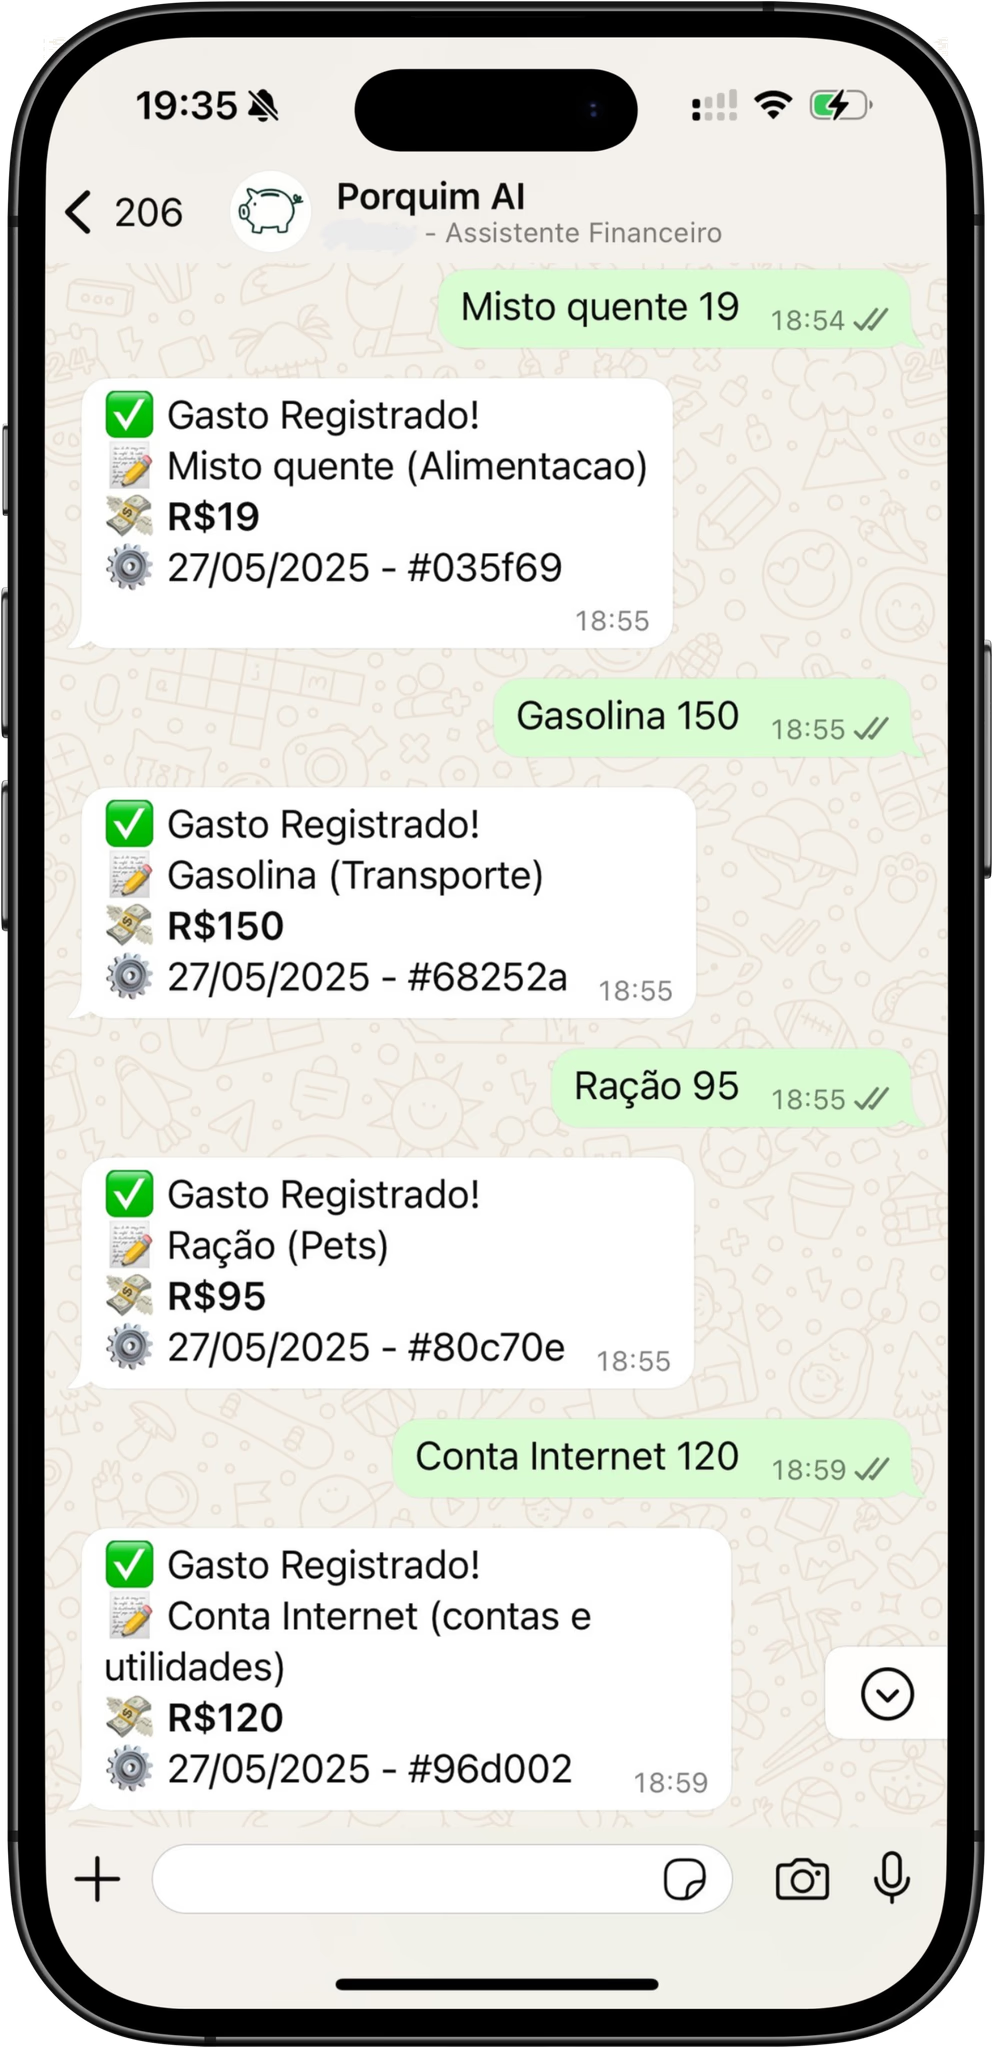
\includegraphics[width=0.8\textwidth,height=0.6\textheight,keepaspectratio]{figs/porquim.png}
    \fonte{\citeonline{porquim_2026}.}
\end{figure}

O \textbf{Ganhos e Gastos} \cite{ganhos_gastos_2026} apresenta uma solução de controle financeiro pessoal baseada na utilização de inteligência artificial e na integração com o WhatsApp. A ferramenta busca facilitar o registro de receitas e despesas, oferecendo recursos destinados à organização das movimentações e à apresentação de informações financeiras de maneira acessível.

Entre as características descritas na pesquisa original estão o lançamento de transações, a categorização de movimentações financeiras e a visualização de informações por meio de gráficos e indicadores. A utilização do WhatsApp como canal de entrada de dados aproxima a ferramenta das atividades cotidianas dos usuários, reduzindo a necessidade de interação constante com interfaces tradicionais de registro.

O GranaAI compartilha dessa abordagem ao utilizar mensagens em linguagem natural para o registro financeiro, mas também contempla o desenvolvimento de uma plataforma web integrada. Essa estrutura busca permitir que os usuários consultem suas informações financeiras em diferentes formatos, combinando a interação conversacional com recursos de visualização e acompanhamento de receitas e despesas.

\begin{figure}[htbp]
    \centering
    \caption{Interface da plataforma Ganhos e Gastos}
    \label{fig:ganhos-gastos}
    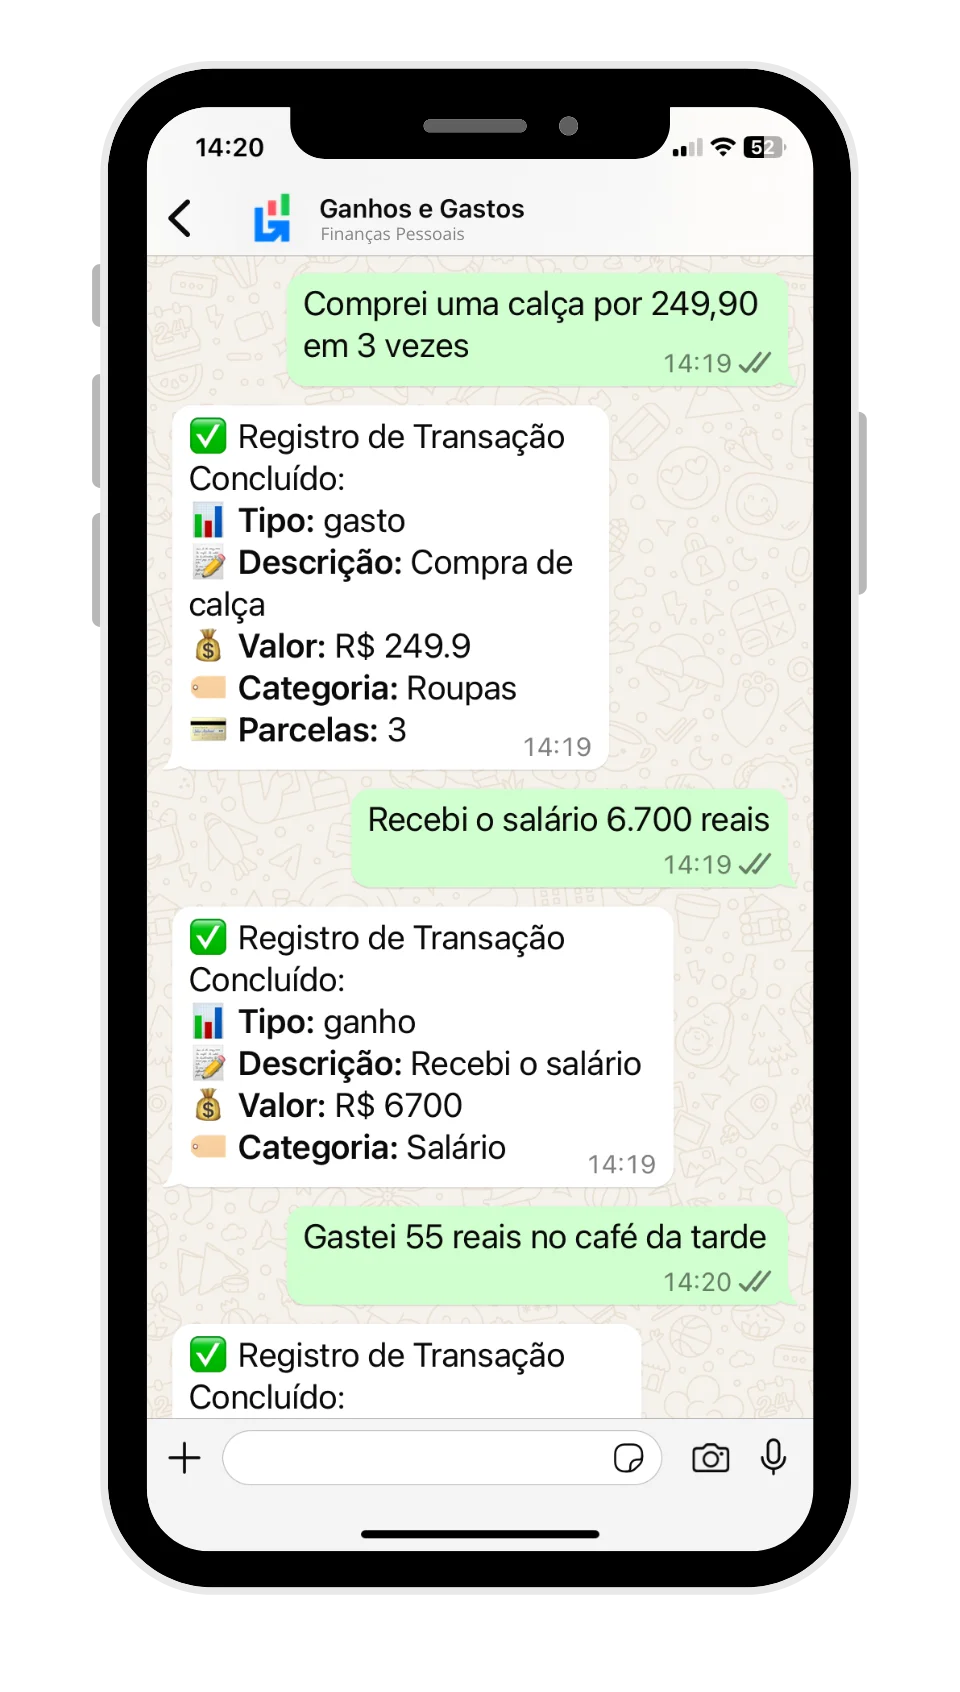
\includegraphics[width=0.8\textwidth,height=0.6\textheight,keepaspectratio]{figs/ganhos-e-gastos.png}
    \fonte{\citeonline{ganhos_gastos_2026}.}
\end{figure}

O \textbf{Lucrefy} \cite{lucrefy_2026} é uma ferramenta voltada ao controle financeiro por meio do WhatsApp, direcionada tanto a pessoas físicas quanto a profissionais autônomos e pequenos negócios. Sua proposta está relacionada à simplificação do acompanhamento de entradas, saídas e resultados financeiros, utilizando uma interface de comunicação familiar aos usuários.

Entre as funcionalidades apresentadas estão o registro de movimentações por conversa, a categorização de gastos, a disponibilização de relatórios e o apoio à separação entre informações financeiras pessoais e profissionais. Essa característica amplia o público potencial da ferramenta, permitindo sua utilização em diferentes contextos de organização financeira.

Diferentemente dessa abrangência, o GranaAI concentra sua proposta no controle financeiro pessoal, com foco no registro e na organização de movimentações individuais. A solução busca integrar a praticidade da comunicação pelo WhatsApp a recursos de acompanhamento financeiro disponibilizados em uma interface web, considerando as necessidades identificadas durante a pesquisa com potenciais usuários.

\begin{figure}[htbp]
    \centering
    \caption{Interface da plataforma Lucrefy}
    \label{fig:lucrefy}
    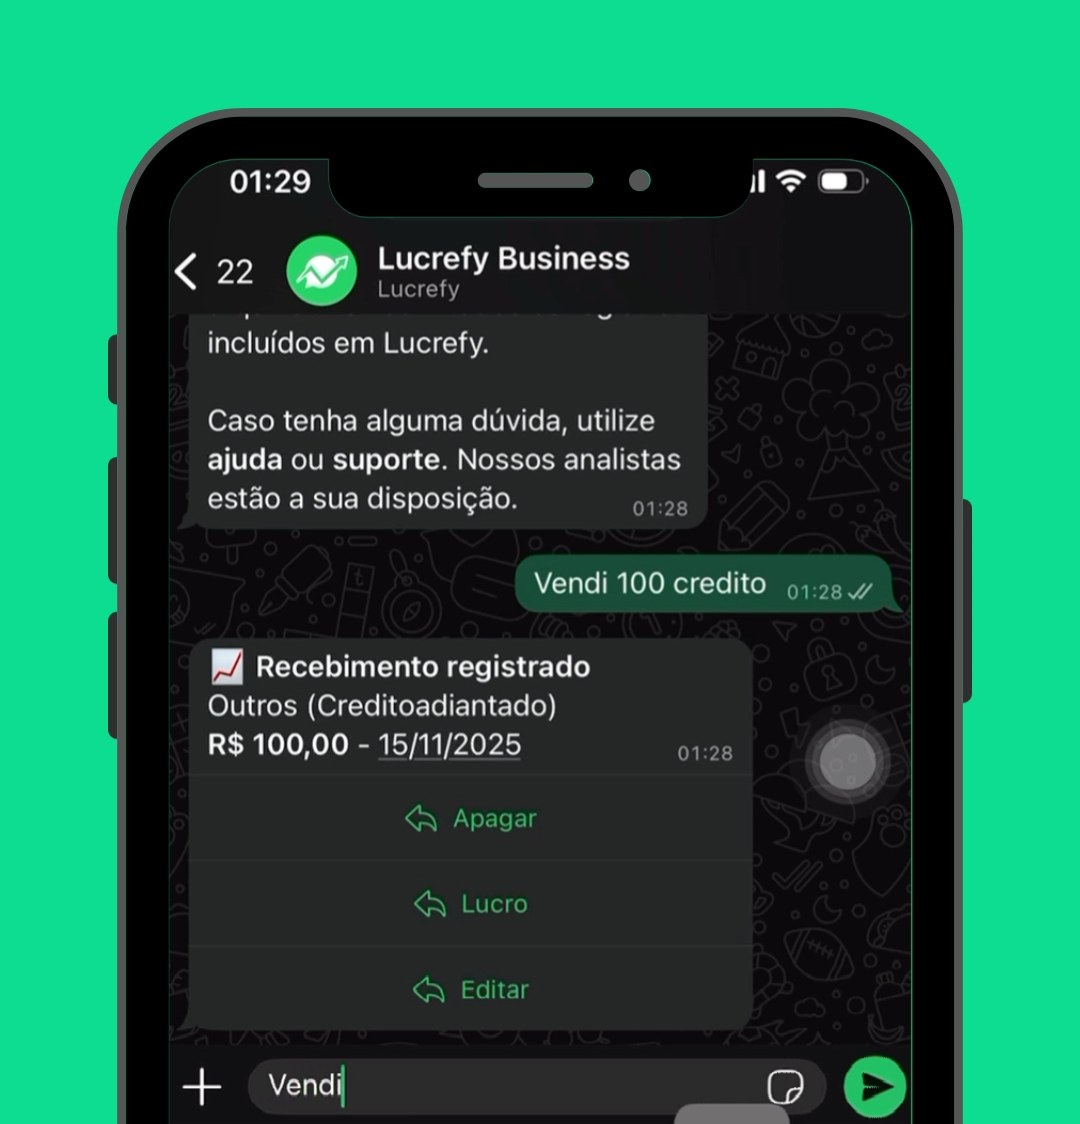
\includegraphics[width=0.8\textwidth,height=0.6\textheight,keepaspectratio]{figs/lucrefy.png}
    \fonte{\citeonline{lucrefy_2026}.}
\end{figure}

O \textbf{Bot Financeiro} \cite{bot_financeiro_2026} utiliza o WhatsApp como principal interface para o registro e o acompanhamento de movimentações financeiras. A ferramenta busca atender usuários que enfrentam dificuldades para registrar suas despesas no momento em que ocorrem, oferecendo alternativas de interação que procuram tornar essa atividade mais rápida e conveniente.

Conforme o levantamento realizado no TCC I, a solução permite o envio de informações por mensagens de texto, áudio ou imagens, utilizando inteligência artificial para interpretar os dados recebidos e organizar as transações financeiras. Também são apresentados recursos de categorização automática e geração de resumos financeiros por período ou categoria, permitindo a consulta de informações relacionadas aos hábitos de consumo.

A análise dessa ferramenta contribui para compreender a utilização de interfaces conversacionais como alternativa aos métodos tradicionais de registro financeiro. No desenvolvimento do GranaAI, essa abordagem é associada a uma plataforma web complementar, destinada à apresentação de indicadores e ao acompanhamento das movimentações armazenadas, permitindo explorar diferentes formas de consulta e organização das informações financeiras.

\begin{figure}[htbp]
    \centering
    \caption{Interface da plataforma Bot Financeiro}
    \label{fig:bot-financeiro}
    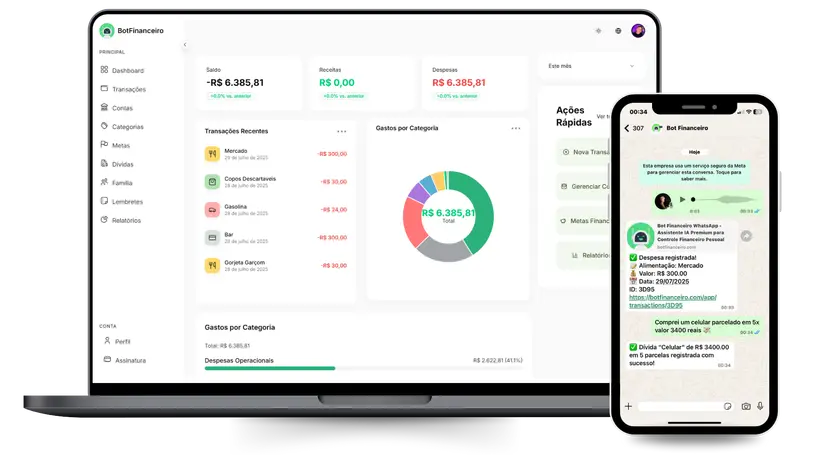
\includegraphics[width=0.8\textwidth,height=0.6\textheight,keepaspectratio]{figs/botfinanceiro.png}
    \fonte{\citeonline{bot_financeiro_2026}.}
\end{figure}

O \textbf{ZapGastos} \cite{zapgastos_2026} apresenta uma solução de assistência financeira integrada ao WhatsApp, com funcionalidades voltadas ao controle de contas, cartões, receitas e despesas. A ferramenta procura simplificar a organização financeira por meio de recursos de registro e acompanhamento das movimentações, reduzindo a dependência de planilhas e procedimentos manuais.

Entre as funcionalidades identificadas no levantamento original estão o lançamento de informações por texto, áudio ou imagem, a edição de transações, o envio de lembretes e a disponibilização de relatórios, gráficos e informações financeiras personalizadas. A pesquisa também descreve a integração com instituições financeiras por meio do Open Finance, recurso que possibilita ampliar a automação na obtenção de dados mediante os procedimentos de autorização aplicáveis.

Essa característica representa uma abordagem distinta daquela adotada inicialmente pelo GranaAI, cuja proposta se concentra no registro de informações fornecidas pelo próprio usuário por meio da interface conversacional. Dessa forma, o sistema desenvolvido neste trabalho busca oferecer uma alternativa de acompanhamento financeiro baseada na interação direta pelo WhatsApp e na organização dos registros em uma plataforma web, sem depender de integração bancária para suas funcionalidades centrais.

\begin{figure}[htbp]
    \centering
    \caption{Interface da plataforma ZapGastos}
    \label{fig:zapgastos}
    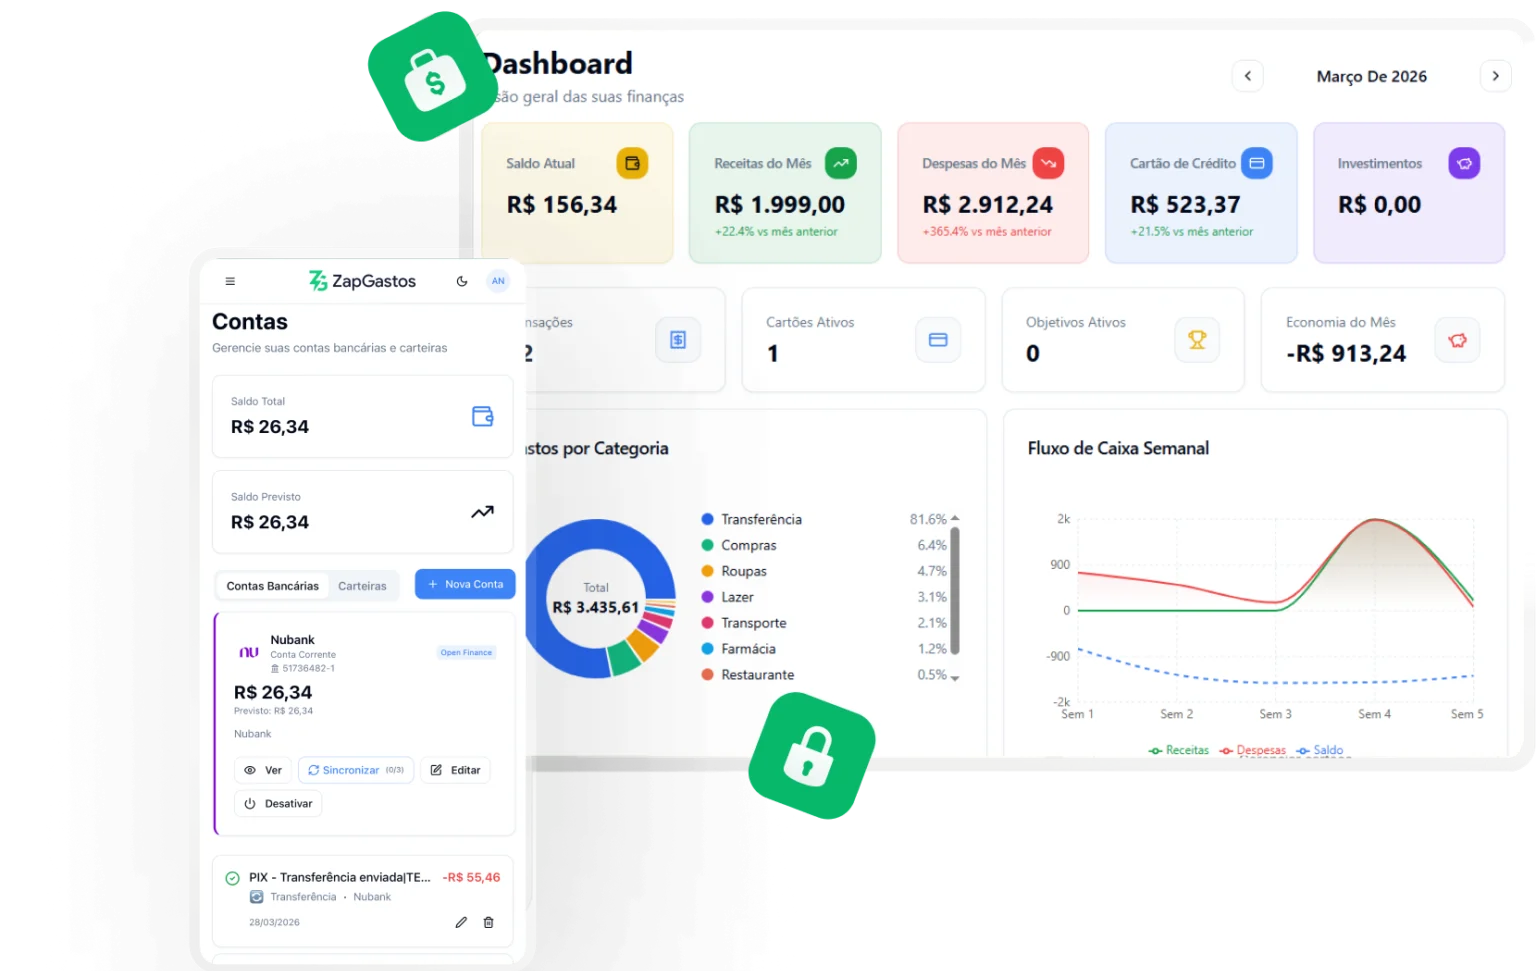
\includegraphics[width=0.8\textwidth,height=0.6\textheight,keepaspectratio]{figs/zapgastos.png}
    \fonte{\citeonline{zapgastos_2026}.}
\end{figure}

A análise das cinco soluções evidencia a utilização de interfaces conversacionais e recursos de inteligência artificial como estratégias recorrentes para facilitar o registro e o acompanhamento de informações financeiras. Apesar das diferenças relacionadas ao público-alvo, às funcionalidades e às formas de apresentação dos dados, as ferramentas analisadas compartilham o objetivo de tornar a organização financeira mais prática e integrada ao cotidiano dos usuários.

Nesse contexto, o GranaAI foi concebido a partir da combinação entre uma interface conversacional integrada ao WhatsApp e uma plataforma web de acompanhamento financeiro. Sua proposta busca reunir o registro de movimentações em linguagem natural e a visualização estruturada das informações em um mesmo sistema, considerando os requisitos identificados durante a pesquisa e as possibilidades tecnológicas investigadas.

A análise dos concorrentes contribuiu, portanto, para fundamentar decisões relacionadas às funcionalidades, à experiência de utilização e à arquitetura da solução, estabelecendo uma referência para o desenvolvimento e a posterior avaliação do GranaAI.

\subsection{Artigos Científicos Relacionados}

A utilização de inteligência artificial em atividades relacionadas ao setor financeiro tem sido objeto de investigações científicas que buscam compreender suas possibilidades de aplicação, seus benefícios e suas limitações. Entre as tecnologias estudadas, destacam-se os grandes modelos de linguagem, também conhecidos como \textit{Large Language Models} (LLMs), capazes de processar informações textuais e produzir respostas em linguagem natural a partir das solicitações dos usuários.

No contexto das finanças pessoais, esses modelos podem ser empregados em atividades de interpretação de informações, esclarecimento de dúvidas, planejamento financeiro e apoio à análise de dados. Entretanto, sua utilização exige atenção à qualidade das respostas geradas, à possibilidade de ocorrência de vieses e à necessidade de distinguir informações de caráter educativo de recomendações financeiras especializadas.

Para fundamentar o desenvolvimento do GranaAI, foram selecionados dois estudos científicos que investigam diferentes aspectos da aplicação de modelos de linguagem em atividades financeiras. O primeiro examina a capacidade desses modelos de produzir recomendações de investimento considerando características individuais. O segundo analisa os padrões de utilização de inteligência artificial generativa em tarefas cotidianas de gestão financeira pessoal.

A análise desses trabalhos contribui para compreender as possibilidades de utilização de interfaces baseadas em linguagem natural e para estabelecer critérios de cautela no desenvolvimento de uma solução tecnológica destinada ao registro, à organização e ao acompanhamento de informações financeiras.

\subsubsection{Uso de modelos de linguagem em aconselhamento financeiro}

O estudo \textit{Using Large Language Models for Financial Advice}, desenvolvido por \citeonline{fieberg2024financialadvice}, investiga a capacidade de grandes modelos de linguagem de produzir recomendações financeiras adequadas às características de diferentes investidores. A pesquisa busca compreender em que medida esses modelos conseguem considerar informações individuais na elaboração de orientações relacionadas à composição de carteiras de investimento, além de identificar características tecnológicas associadas à qualidade das recomendações geradas.

Para a realização do estudo, os pesquisadores analisaram recomendações produzidas por 32 modelos de linguagem, considerando 64 perfis de investidores. Esses perfis foram construídos a partir de características como preferência por risco, país de origem, preferências relacionadas à sustentabilidade, gênero e experiência com investimentos. A utilização de diferentes combinações permitiu investigar a capacidade dos modelos de adaptar suas respostas às condições apresentadas.

Os resultados indicaram que os modelos de linguagem analisados demonstraram capacidade de considerar características relevantes dos investidores na elaboração de recomendações financeiras. Os autores observaram que determinados modelos apresentaram maior sensibilidade às informações individuais e produziram sugestões com características compatíveis com os perfis avaliados.

Entretanto, a pesquisa também identificou limitações importantes, especialmente relacionadas à reprodução de vieses presentes no comportamento humano. Entre os aspectos observados, destaca-se a tendência de favorecer ativos associados ao país de origem do investidor, fenômeno conhecido como \textit{home bias}. Esse resultado demonstra que, embora os modelos de linguagem possam apresentar respostas tecnicamente plausíveis, suas recomendações não estão necessariamente livres de distorções.

A contribuição desse estudo para o desenvolvimento do GranaAI está relacionada à compreensão das possibilidades e limitações dos modelos de linguagem na interpretação de informações financeiras. Embora a pesquisa de \citeonline{fieberg2024financialadvice} esteja direcionada ao aconselhamento de investimentos, seus resultados oferecem fundamentos para discutir o emprego de inteligência artificial em aplicações que processam informações fornecidas pelos usuários e produzem respostas contextualizadas.

No GranaAI, essa discussão é especialmente relevante porque o sistema utiliza inteligência artificial em uma interface conversacional destinada ao controle financeiro pessoal. A utilização de modelos de linguagem pode facilitar a interpretação de mensagens e a interação com informações financeiras, mas também exige cuidados relacionados à precisão dos dados e à confiabilidade das respostas apresentadas.

Dessa forma, o estudo reforça a importância de compreender a inteligência artificial como um recurso de apoio ao processamento e à apresentação de informações, sem pressupor que suas respostas sejam sempre corretas ou equivalentes à orientação de um profissional especializado.

\subsubsection{Uso de IA generativa na gestão financeira pessoal}

O artigo \textit{How Individuals Use Generative AI for Personal Financial Management}, publicado por \citeonline{pak2026personalfinance} no periódico \textit{Journal of Behavioral and Experimental Finance}, investiga como indivíduos utilizam ferramentas de inteligência artificial generativa em diferentes atividades relacionadas à administração de suas finanças pessoais.

A pesquisa foi realizada com dados de 2.170 adultos sul-coreanos, com idades entre 25 e 59 anos, considerando dez áreas de utilização da inteligência artificial: elaboração de orçamentos, planejamento de poupança, investimentos, questões tributárias, gerenciamento de dívidas, seguros, moradia, identificação de fraudes, educação financeira e apoio psicológico relacionado a questões financeiras.

Os resultados demonstraram que 67,8\% dos participantes haviam utilizado modelos de linguagem para pelo menos uma atividade financeira, enquanto 58,7\% relataram sua utilização em duas ou mais áreas. Além disso, aproximadamente 15\% dos respondentes informaram ter utilizado essas tecnologias em todas as dez categorias investigadas.

Entre as aplicações mais frequentes, destacaram-se o uso de inteligência artificial para investimentos em ações, mencionado por 50,3\% dos participantes, o planejamento de poupança, com 48,2\%, a elaboração e o acompanhamento de orçamentos, com 47,6\%, e as atividades relacionadas à declaração e ao planejamento tributário, com 46,5\%.

O estudo também identificou diferentes formas de interação com os modelos de linguagem. Parte dos participantes utilizava essas ferramentas como recursos educativos para compreender conceitos e procedimentos financeiros, enquanto outros recorriam à inteligência artificial para pesquisar informações, comparar alternativas e obter apoio em determinadas decisões. Em alguns casos, os modelos também eram utilizados como fontes de suporte diante de preocupações relacionadas às finanças.

Esses resultados evidenciam a diversidade de aplicações da inteligência artificial generativa na gestão financeira pessoal, demonstrando que sua utilização não se restringe a atividades complexas de investimento, mas também abrange tarefas relacionadas ao planejamento, à organização e ao acompanhamento de recursos financeiros.

A contribuição do estudo de \citeonline{pak2026personalfinance} para o GranaAI está relacionada à identificação de usos concretos de modelos de linguagem em atividades financeiras cotidianas. A pesquisa fornece evidências de que essas tecnologias já são utilizadas por parte dos indivíduos para buscar informações e apoiar tarefas de organização financeira, aspecto que se aproxima da proposta de desenvolver uma solução baseada em interação conversacional.

Entretanto, é importante observar que a investigação foi conduzida com participantes da Coreia do Sul, em um contexto social, econômico e tecnológico específico. Dessa forma, seus resultados não devem ser generalizados diretamente para a população brasileira, embora ofereçam referências relevantes para a compreensão das possibilidades de aplicação da inteligência artificial generativa.

No desenvolvimento do GranaAI, a utilização do WhatsApp como interface conversacional busca explorar essas possibilidades em um ambiente de comunicação familiar aos usuários, enquanto a plataforma web complementa a interação por meio da apresentação estruturada das informações financeiras registradas.

Assim, o estudo contribui para fundamentar a escolha de uma abordagem tecnológica que combina linguagem natural, organização de dados e acompanhamento financeiro, sem pressupor que a adoção da ferramenta, por si só, produza melhorias comprovadas no comportamento financeiro dos usuários.

Em conjunto, os estudos de \citeonline{fieberg2024financialadvice} e \citeonline{pak2026personalfinance} demonstram diferentes perspectivas sobre a utilização de grandes modelos de linguagem em atividades financeiras. Enquanto o primeiro investiga a adequação e as limitações das recomendações produzidas por essas tecnologias, o segundo examina sua utilização prática por indivíduos em diferentes tarefas de gestão financeira pessoal.

Essas contribuições oferecem fundamentos para o desenvolvimento do GranaAI, especialmente quanto à aplicação de inteligência artificial em interfaces conversacionais, à necessidade de confiabilidade das informações processadas e à importância de compreender as tecnologias como instrumentos de apoio à organização financeira pessoal.

\section{Tecnologias}

O desenvolvimento de sistemas de informação envolve a seleção e a integração de tecnologias capazes de atender aos requisitos funcionais e não funcionais estabelecidos durante as etapas de análise e planejamento. A escolha dessas tecnologias deve considerar aspectos como compatibilidade entre componentes, facilidade de manutenção, possibilidades de integração, organização da arquitetura e adequação às necessidades dos usuários.

No contexto do GranaAI, a definição das tecnologias utilizadas esteve relacionada à necessidade de construir uma solução capaz de receber informações financeiras por meio de uma interface conversacional, interpretar mensagens em linguagem natural, processar e armazenar movimentações financeiras e disponibilizar os dados registrados em uma plataforma web.

Para atender a essas necessidades, a solução contempla diferentes componentes tecnológicos, organizados de acordo com suas responsabilidades no funcionamento do sistema. A integração com o WhatsApp permite estabelecer um canal de comunicação entre o usuário e a aplicação, enquanto os serviços de backend são responsáveis pelo processamento das requisições, pela execução das regras de negócio e pela comunicação com os demais recursos utilizados.

A utilização de modelos de linguagem, disponibilizados por meio de uma interface de programação de aplicações, possibilita incorporar recursos de inteligência artificial ao processamento de mensagens. Complementarmente, o emprego de um sistema gerenciador de banco de dados relacional permite estruturar e persistir as informações financeiras, enquanto as tecnologias de desenvolvimento web viabilizam a construção de uma interface destinada à consulta e à visualização dos registros.

Entre as tecnologias consideradas no desenvolvimento do GranaAI, destacam-se o WhatsApp, a Evolution API, a linguagem Python, o framework FastAPI, a Groq API, o Docker, o JavaScript, o TypeScript, o React, o Node.js e o PostgreSQL. Também são utilizados recursos complementares para validação de dados e comunicação com o banco de dados, como Pydantic e SQLAlchemy.

A seleção dessas tecnologias está associada à possibilidade de organizar a aplicação em componentes com responsabilidades específicas, favorecendo a separação entre a interface de comunicação, o processamento das informações, a persistência dos dados e a apresentação dos resultados ao usuário.

Nas subseções seguintes, são apresentados os conceitos, as características e as principais funcionalidades dessas tecnologias, buscando estabelecer a fundamentação necessária para compreender sua utilização no GranaAI. A descrição detalhada da arquitetura, das integrações e das decisões de implementação será apresentada posteriormente, no capítulo dedicado ao desenvolvimento do sistema.

\subsection{WhatsApp}

O WhatsApp é uma plataforma de comunicação instantânea que permite a troca de mensagens de texto, áudios, imagens, vídeos e documentos, além da realização de chamadas de voz e vídeo. Sua utilização em diferentes contextos de comunicação pessoal e profissional possibilita a interação entre indivíduos e organizações por meio de uma interface baseada em conversas, caracterizada pela troca direta de informações entre os participantes.

Além das funcionalidades destinadas à comunicação cotidiana, a plataforma disponibiliza recursos voltados à integração com sistemas externos. Nesse contexto, a WhatsApp Business Platform oferece mecanismos para o envio e o recebimento de mensagens por meio de interfaces de programação de aplicações, permitindo que desenvolvedores construam soluções capazes de automatizar determinados processos de comunicação \cite{whatsapp_cloud_api_2026}.

Entre os mecanismos utilizados nessas integrações, destacam-se as APIs e os webhooks. As APIs permitem que aplicações externas realizem operações disponibilizadas por um serviço, enquanto os webhooks possibilitam o envio de notificações relacionadas à ocorrência de eventos específicos. No contexto de plataformas de mensagens, esses mecanismos podem ser utilizados para receber informações sobre novas mensagens e encaminhá-las aos serviços responsáveis pelo processamento das solicitações \cite{whatsapp_cloud_api_2026}.

A utilização de aplicativos de mensagens como interface de sistemas de informação apresenta possibilidades de aplicação em atividades que exigem interação frequente com os usuários. Em soluções de controle financeiro pessoal, essa abordagem pode permitir que informações relacionadas a receitas e despesas sejam fornecidas diretamente em uma conversa, reduzindo a necessidade de acessar diferentes telas para realizar registros cotidianos.

No desenvolvimento do GranaAI, o WhatsApp foi selecionado como canal de interação conversacional entre o usuário e o sistema. A proposta consiste em permitir que movimentações financeiras sejam informadas por meio de mensagens em linguagem natural, possibilitando seu encaminhamento aos componentes responsáveis pela interpretação, pelo processamento e pelo armazenamento dos dados.

A integração entre o WhatsApp e os serviços internos do GranaAI é realizada com o auxílio da Evolution API, apresentada na subseção seguinte. Essa ferramenta atua como intermediária na comunicação entre a plataforma de mensagens e a aplicação, permitindo que os eventos recebidos sejam encaminhados ao backend responsável pela execução das funcionalidades financeiras.

Dessa forma, o WhatsApp constitui um dos principais componentes da interface de interação do GranaAI, enquanto os processos de interpretação das mensagens, validação das informações e persistência dos registros são executados pelos demais serviços que compõem a arquitetura da solução.

\subsection{Evolution API}

A Evolution API é uma interface de programação de aplicações, baseada na arquitetura \textit{Representational State Transfer} (REST), desenvolvida para possibilitar a integração entre o WhatsApp e sistemas externos. Sua principal finalidade é disponibilizar recursos que permitam o gerenciamento de conexões, o envio e o recebimento de mensagens e a comunicação automatizada entre diferentes serviços computacionais. Dessa forma, a ferramenta pode ser utilizada no desenvolvimento de aplicações que necessitam incorporar funcionalidades de comunicação por meio do WhatsApp \cite{evolution_api_docs_2026}.

De acordo com sua documentação, a Evolution API integra o ecossistema Evolution e oferece suporte a diferentes mecanismos de conexão, incluindo tecnologias como Baileys e a Meta Business API. A ferramenta foi desenvolvida utilizando Node.js e TypeScript, tecnologias que possibilitam a construção de serviços voltados à comunicação entre aplicações e ao processamento de requisições \cite{evolution_api_docs_2026}.

Entre suas principais funcionalidades, destacam-se os recursos de gerenciamento de instâncias, envio de mensagens, consulta de informações de contatos e grupos e disponibilização de eventos relacionados às interações realizadas na plataforma. O gerenciamento de instâncias permite organizar conexões utilizadas pelos sistemas integrados, enquanto os endpoints REST oferecem operações que podem ser acionadas por aplicações externas por meio de requisições HTTP.

Outro recurso relevante da Evolution API é a utilização de webhooks, mecanismos que permitem encaminhar notificações a sistemas externos quando determinados eventos são identificados. Em aplicações conversacionais, esses eventos podem estar relacionados ao recebimento de mensagens, às atualizações de conexão e a outras ocorrências associadas à comunicação. Dessa maneira, a aplicação responsável pelo processamento das informações pode receber notificações sem depender exclusivamente de consultas periódicas ao serviço de mensagens.

A arquitetura baseada em eventos apresenta possibilidades importantes para o desenvolvimento de sistemas automatizados, pois permite organizar o processamento das informações em etapas. Quando uma mensagem é recebida, por exemplo, o serviço de integração pode encaminhar os dados para uma aplicação externa, que realiza as operações necessárias e, posteriormente, utiliza os recursos da API para enviar uma resposta ao usuário.

Além dessas funcionalidades, a documentação da Evolution API apresenta possibilidades de integração com ferramentas como Typebot, Chatwoot, OpenAI, Dify, n8n e Flowise, demonstrando sua aplicação em diferentes cenários de automação e desenvolvimento de interfaces conversacionais \cite{evolution_api_docs_2026}.

No contexto do GranaAI, a Evolution API desempenha o papel de componente intermediário entre o WhatsApp e os serviços internos da aplicação. Sua utilização está relacionada à necessidade de receber mensagens enviadas pelos usuários e encaminhar as informações ao backend, responsável pelo processamento das solicitações e pela execução das regras de negócio do sistema.

A partir dessa integração, mensagens relacionadas ao registro de receitas e despesas podem ser encaminhadas aos componentes responsáveis pela interpretação das informações financeiras. Após o processamento, a aplicação pode utilizar os mecanismos de comunicação disponibilizados pela Evolution API para retornar respostas ao usuário por meio do próprio WhatsApp.

É importante destacar que a Evolution API não é responsável, isoladamente, pela interpretação semântica das mensagens ou pelo gerenciamento das informações financeiras. Essas atividades pertencem aos demais componentes do GranaAI, incluindo os serviços de backend, os recursos de inteligência artificial e o sistema de armazenamento de dados. Assim, a ferramenta atua principalmente na camada de integração e comunicação.

Dessa forma, a utilização da Evolution API contribui para a organização da arquitetura do GranaAI, permitindo separar as responsabilidades relacionadas à comunicação com o WhatsApp daquelas associadas ao processamento das mensagens e à execução das funcionalidades financeiras. Essa separação favorece a modularização do sistema e estabelece uma estrutura de integração que pode ser analisada e aprimorada durante as etapas de desenvolvimento e manutenção da aplicação.

\subsection{Chatbot}

\subsection{n8n}

\subsection{Groq API}

\subsection{Docker}

\subsection{JavaScript}

\subsection{React}

\subsection{Node.js}

\subsection{PostgreSQL}
